\documentclass [a4paper, 12pt]{article}

%\usepackage[utf8]{inputenc}
%\usepackage{amssymb}
%\usepackage{amsmath}
%\usepackage{bm}
%\usepackage{epsfig}
%\usepackage{graphicx}
%\usepackage{times}
%\usepackage{float}
%\usepackage[usenames,dvipsnames]{color}
%\usepackage{caption}
%\usepackage[caption=false]{subfig}
%\usepackage{hyperref}
%\usepackage{cleveref}
%\usepackage[version=4]{mhchem}

\usepackage{mathptmx}       % selects Times Roman as basic font
\usepackage{helvet}         % selects Helvetica as sans-serif font
\usepackage{courier}        % selects Courier as typewriter font
\usepackage{type1cm}        % activate if the above 3 fonts are
                            % not available on your system
\usepackage{makeidx}         % allows index generation
\usepackage{graphicx}        % standard LaTeX graphics tool
                             % when including figure files
\usepackage{multicol}        % used for the two-column index
\usepackage[version=4]{mhchem}
\usepackage{cleveref}
\usepackage[usenames,dvipsnames]{xcolor}
\usepackage{bm}
\usepackage[caption=false]{subfig}
%\usepackage{textcomp}
\usepackage{tikz}
\usetikzlibrary{decorations.markings}
\usetikzlibrary{shapes.misc,shapes.geometric,arrows,positioning,automata, patterns}
\usepackage{sidecap}
\usepackage{placeins}


\textwidth 16 cm
\textheight 23 cm
\setlength{\oddsidemargin}{0.1 cm}
\setlength{\topmargin}{1 cm}
\setlength{\headheight}{0cm}
\setlength{\headsep}{0cm}
\setlength{\footskip}{0.75cm}
\setlength{\parindent}{0cm}
\setlength{\oddsidemargin}{0.1 cm}
\setlength{\itemsep}{10pt}
\bibliographystyle{gcs}

\DeclareUnicodeCharacter{2212}{-}
\newcommand{\matr}[1]{\bm{\mathit{#1}}}
\newcommand{\beq}{\begin{equation}}
\newcommand{\eeq}{\end{equation}}
\begin{document}
 
\begin{figure}[h!]
\begin{center}
  
\includegraphics[scale=0.45]{Figures/GCS-hlrs-fzj-lrz.jpg}\\
\end{center}
\end{figure}

\begin{center}
{\LARGE \bf Request for a Project Extension} \\

\bigskip
\bigskip
\bigskip
\end{center}
\textbf{Extended period}\\
\phantom{MM}\textit{01.11.2017-30.06.2019}

\bigskip
\textbf{Project title}\\
\phantom{MM}\textit{KKRnano: Quantum description of skyrmions in chiral B20 magnets}

%\bigskip
%\textbf{Type of project}\\
%\phantom{MM} \textit{new project}

\bigskip
\textbf{Project ID}\\
\phantom{MM} \textit{GCS-KKRN}

\bigskip
\textbf{Principal investigator}\\
\phantom{MM} \textit{ Prof. Dr. Stefan Bl{\"u}gel,
Institute for Advanced Simulation and Peter Gr\"unberg Institut, Forschungszentrum J\"ulich, D-52425 J\"ulich, Germany
}

\bigskip
\textbf{Project contributor(s)}\\

\phantom{MM} \textit{Marcel Bornemann,
Institute for Advanced Simulation and Peter Gr\"unberg Institut, Forschungszentrum J\"ulich, D-52425 J\"ulich, Germany
}

\phantom{MM} \textit{Dr. Sergii Grytsiuk,
Institute for Advanced Simulation and Peter Gr\"unberg Institut, Forschungszentrum J\"ulich, D-52425 J\"ulich, Germany
}

\phantom{MM} \textit{Dr. Roman Kováčik,
Institute for Advanced Simulation and Peter Gr\"unberg Institut, Forschungszentrum J\"ulich, D-52425 J\"ulich, Germany
}


\phantom{MM} \textit{Dr. Rudolf Zeller,
Institute for Advanced Simulation and Peter Gr\"unberg Institut, Forschungszentrum J\"ulich, D-52425 J\"ulich, Germany
}

%\phantom{MM} \textit{Dr. Paul F. Baumeister,
%Institute for Advanced Simulation and J\"ulich Supercomputing Centre, Forschungszentrum J\"ulich, D-52425 J\"ulich, Germany
%}


\newpage

%\vfill
%\tableofcontents
%\vfill

%\newpage

\section{Introduction}
\label{sec:intro}
We have developed a unique electronic structure code based on Density Functional Theory, 
KKRnano \cite{zeller_towards_2008,thiess_massively_2012,bornemann_large-scale_nodate},
specifically designed for petaFLOP computing. Our method scales linearly
with the number of atoms, so that we can realize system sizes of up to 
half a million atoms in a unit cell if necessary.
Recently, we generalized the algorithm to the vectorial spin density formulation enabling us
to calculate complex non-collinear magnetic structures. We implemented a relativistic 
generalization  of our algorithm  such that we are able to treat skyrmions,
in real space. Skyrmions are two-dimensional magnetization solitons, i.e., two-dimensional
magnetic structures localized in space, topologically protected by a non-trivial
magnetization texture, which has particle-like properties. Necessary condition for the 
emergence of skyrmions is the spin-orbit interaction in magnets with broken inversion symmetry.
Chiral magnetic B20 compounds are cubic crystals fulfilling the conditions above. 
The focus of our work is on the germanide \ce{MnGe} that is particularly
interesting among the chiral magnetic B20 compounds, as it exhibits a three-dimensional magnetic structure
that is not yet understood (see preliminary results
\cite{tanigaki_real-space_2015,rybakov_new_2016,bornemann_investigation_2017,bornemann_large-scale_2018}).

Due to the unexpected challenges mentioned below,
we request an extension of the project period until 30th June 2019.


\section{Complex Magnetic Textures in B20-\ce{MnGe}}
\label{sec:mnge}

B20-\ce{MnGe} is currently the subject of extensive
investigation
\cite{kanazawa_large_2011,kanazawa_possible_2012,grigoriev_chiral_2013,tanigaki_real-space_2015,martin_magnetic_2016}.
This is mainly inspired by the discovery of skyrmions as small information-carrying particles
that could potentially be used in spintronic devices \cite{fert_magnetic_2017}.
In a recent study \cite{tanigaki_real-space_2015}, it was 
found by transmission electron microscopy that 3D magnetic
objects exist in B20-\ce{MnGe}. The authors of \cite{tanigaki_real-space_2015}
came to the conclusion that their data indicates a
cubic lattice of skyrmionic hedgehogs
and anti-hedgehogs (see \cref{fig:mnge_3q}) 
with a lattice constant of about 3-6 nm.
The singularity at the center of the texture exists only in the micromagnetic description since the
atomic magnetic moment of the atom, which is located at the center,
remains finite \cite{feldtkeller_continuous_2017}.
\begin{figure}[htb]
	\subfloat[]{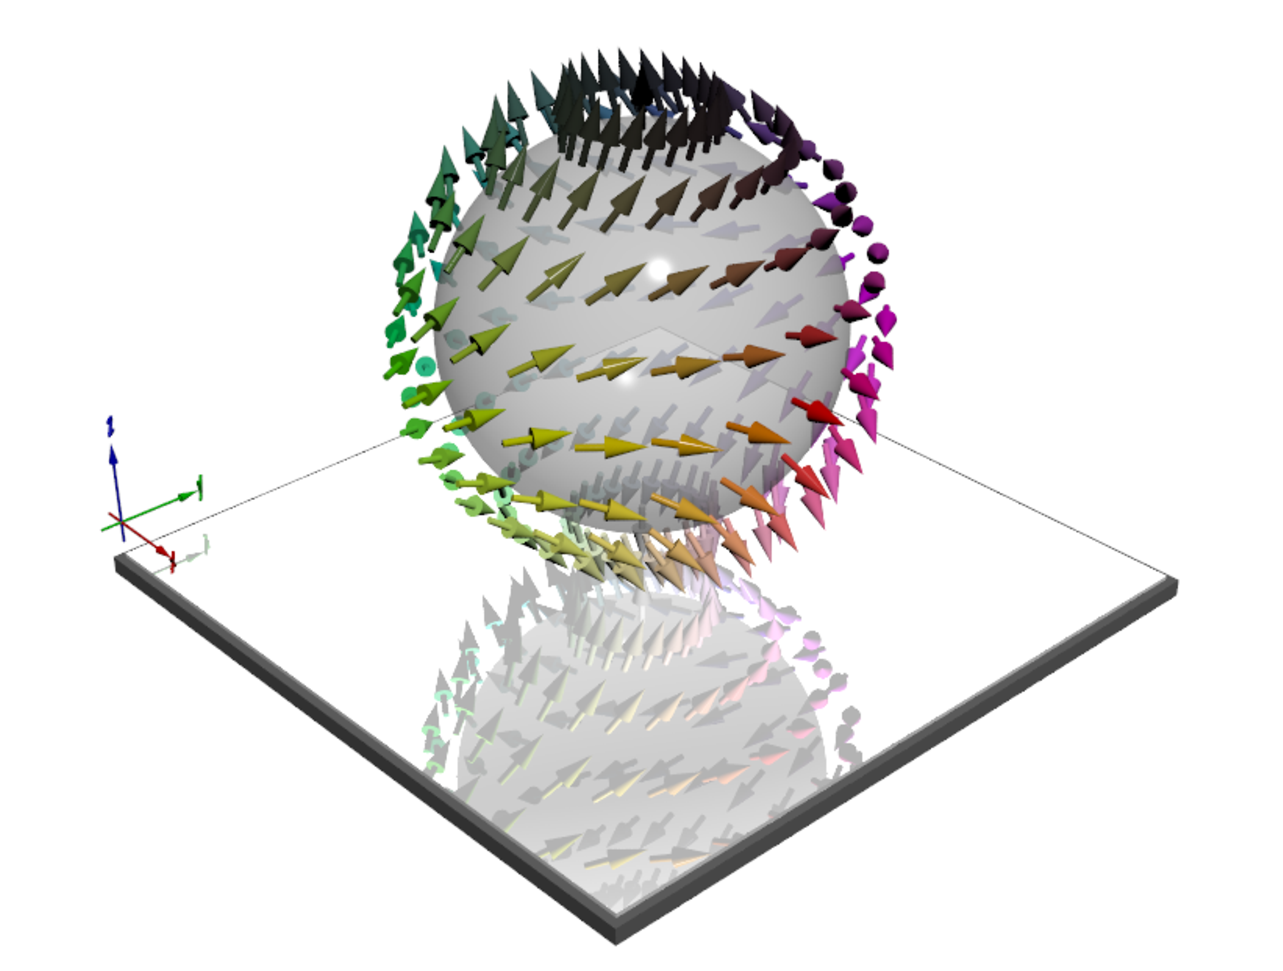
\includegraphics[width=.50\textwidth]{Figures/antihedgehog.eps}\label{fig:mnge_3q}}
	\hfill
	\subfloat[]{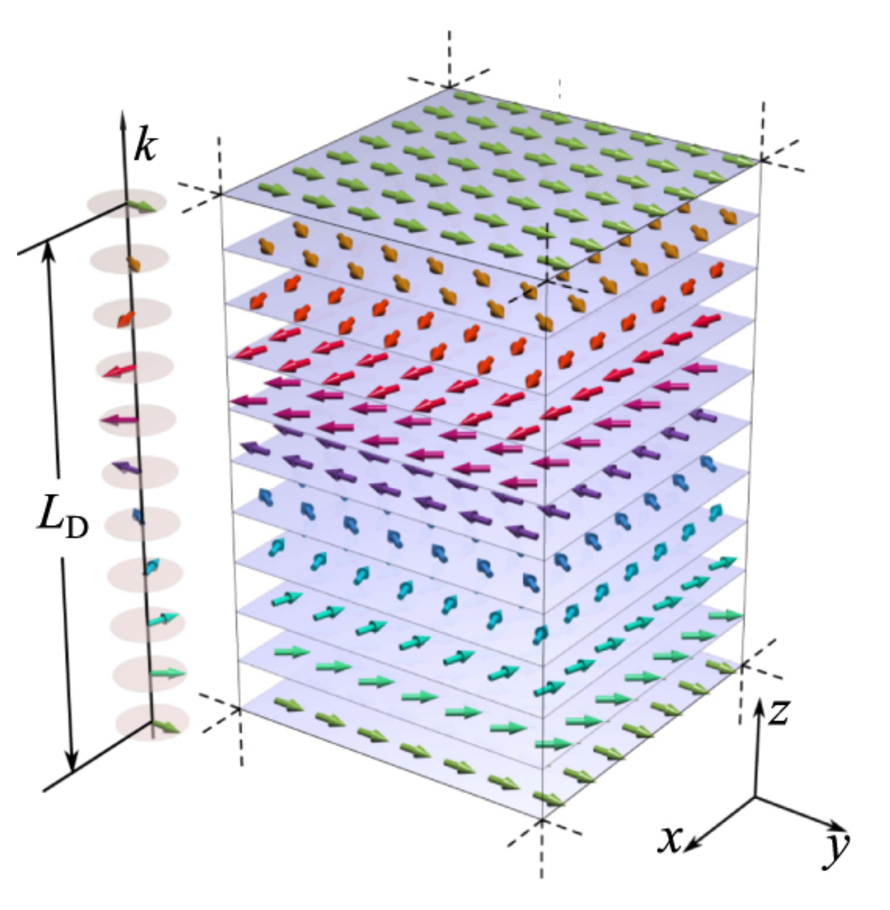
\includegraphics[width=.50\textwidth]{Figures/helicalspiral.eps}\label{fig:mnge_spiral}}
	\hfill
 \caption{Magnetic textures that are found experimentally in B20-\ce{MnGe}: (a) 
	Magnetic anti-hedgehog texture that is wrapped around a singularity at the center.
	Reprinted with kind permission of Nikolai Kiselev. (b) Helical
	spin spiral that propagates in (001) direction. Reprinted from \cite{rybakov_new_2016} and
	licensed under CC BY 3.0.}
\end{figure}
Findings by Kanazawa \textit{et al.}\ suggest that the lattice is set up by a superposition of three orthogonal
helical structures, also referred to as 3Q state \cite{kanazawa_noncentrosymmetric_2017}. 
Here, the local magnetization is determined by the provision
\beq
\label{eq:3q_formula}
\vec{M}(\vec{r}) =
\begin{pmatrix}
	\sin{qy} + \cos{qz} \\
	\sin{qz} + \cos{qx} \\
	\sin{qx} + \cos{qy}
\end{pmatrix},
\eeq
where $q=\frac{2\pi}{\lambda}$ is the wavenumber given in terms of the helical wavelength $\lambda$ and
$x$, $y$ and $z$ are the spatial coordinates within the unit cell.
Note, that $\vec{M}(\vec{r})$ is not normalized.

At present there is a lack of a convincing explanation
of what is observed in experiment. Research in the framework of micromagnetic models identified both
magnetic frustration (RKKY interaction) as well as spin-orbit coupling induced Dzyaloshinskii-Moriya (DM)
interaction as potentially crucial to a better
understanding \cite{altynbaev_hidden_2016,koretsune_control_2015}. 
While the 3Q state certainly constitutes the most interesting non-trivial magnetic texture 
in B20-\ce{MnGe}, there are also reports that the magnetic ground state in this system is
actually a helical spiral (see \cref{fig:mnge_spiral}) \cite{yaouanc_magnetic_2017} which was observed up
to a temperature of 170 K \cite{makarova_neutron_2012}.
These two observations are clearly contradictory and it has not yet been explained how
both can coexist within the same material.
The helical spin spiral in B20-\ce{MnGe} forms along the (001) direction and therefore the magnetization
is described by the relation
\beq
\label{eq:1q_spiral}
\vec{M}(\vec{r}) =
\begin{pmatrix}
	 \cos{qz} \\
	-\sin{qz}  \\
	0
\end{pmatrix}
.
\eeq
In the following, we refer to this as the 1Q state.

In summary, B20 MnGe exhibits a non-understood three-dimensional magnetic structure,
that is different to the ones of the other chiral magnetic B20 systems, \textit{e.g.}\ FeGe,
exhibiting two-dimensional magnetic structures.  No large-scale DFT calculation  has been performed.
However, the relatively short  helical wavelength in B20-\ce{MnGe}  of 3--6~nm makes it ideal to perform
a complete Density Functional Theory (DFT) 
study with KKRnano, without involving a multiscale approach bridging length scales by atomistic spin models. 
Thus, B20-\ce{MnGe} was identified as a prime candidate material to be investigated with the new
version of KKRnano, since it  now contains the feature of non-collinear magnetism and spin-orbit coupling.


\section{Selected Preliminary Results}

In the following we present selected results of our investigations which give an impression
of what has been achieved so far and which questions are still unanswered.
All results are obtained using a $6\times 6\times 6$ B20-\ce{MnGe} supercell (1728 atoms) with 
PBEsol as exchange correlation functional
and we include only a single k-point, \textit{i.e.}, the $\Gamma$-point.
\\
In an initial comparison of ferromagnetic (FM), 1Q and 3Q state the respective states are imposed on
the system by forcing the atomic exchange-correlation B-fields
to point into specific directions. 
For the equilibrium lattice constant
$a=4.80$ \AA, the ferromagnet is the state with the lowest total energy.
As this contradicts experimental observations, we take into consideration that
in experiment the crystal structure might inadvertently differ from the ideal structure.
Such discrepancies can for instance be caused by strain that 
originates from the manufacturing process of the sample.
Therefore, it is reasonable to check whether the material's magnetic properties change, when the
lattice constant is varied.
\begin{figure}[htb]
  \centering
   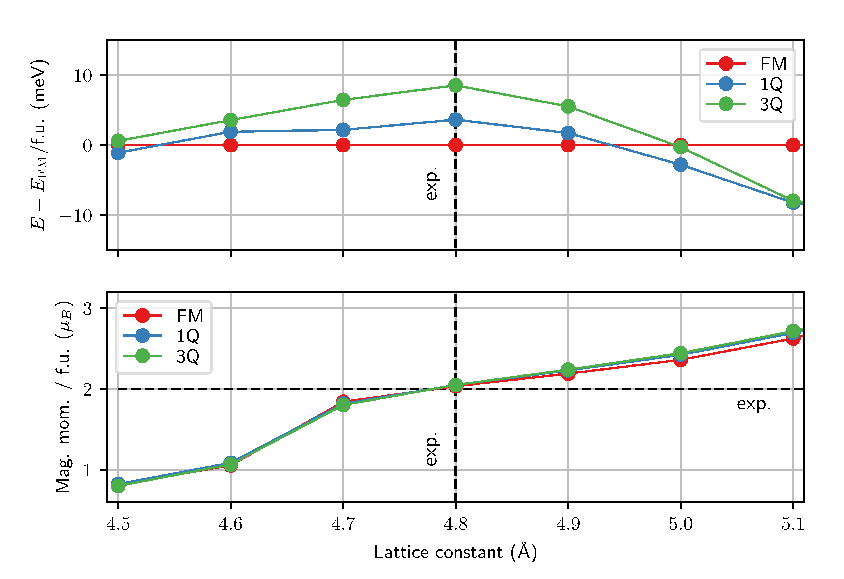
\includegraphics[width=1.00\textwidth]{Figures/MnGe_ferro_1q.eps}
	\caption{Comparison of Ferromagnetic (FM), helical spiral (1Q) and hedgehog lattice (3Q) 
	state with KKRnano.
	Top: Difference of total energies with the FM state as reference state for different
	lattice constants. The experimental lattice constant is $a=4.80$ \AA. 1Q and 3Q state
	are energetically preferable for $a > 5.0$ \AA.
	Bottom: Magnetic moment per \ce{Mn} atom increases with lattice constant.
	High-spin/Low-spin transition is clearly visible between $a=4.60$ and $a=4.70$ \AA.
	Experimentally, the magnetic moment is measured to be $\approx 2 \mu_B$.
}
\label{fig:MnGe_kkrnano_comparison}
\end{figure}
The results of such a variation is displayed in the upper part of \cref{fig:MnGe_kkrnano_comparison}, where
the total energy is evaluated for FM, 1Q and 3Q state as function of the lattice constant.
Clearly, neither the 1Q nor the 3Q state constitutes the ground state,
when the experimental lattice constant is assumed.
Yet, by increasing or decreasing the lattice constant the energetic difference can be made
smaller.
We focus on an increase of the lattice constant rather than a decrease since 
the system goes into the low-spin state below $a=4.65$ \AA \, \cite{rosler_ab_2012} and according to experiment
the non-trivial textures
exist in the high-spin regime.
A crucial transition point is found around $a=5.0$ \AA,
where by imposing the 1Q or 3Q state the energy can be made smaller than for the ferromagnetic state.
In general, for $a>5.0$ \AA \, both helical states are favored over the ferromagnetic one.
Obviously, an artificial increase of the lattice constant by
$0.2$ \AA \, ($\approx 4 \%$) or more is fairly large.
However, experimental samples are seldom if ever perfectly clean and
impurities in the sample need to be considered as a source of error in the
final analysis. One potential
effect of impurities is chemical pressure that causes a spatial expansion of the
lattice structure.
An example of the possible effects of positive chemical pressure
can be found in \ce{Co}-doped B20-\ce{FeGe} \cite{stolt_chemical_2018}. 
Here, it was experimentally observed
that doping can increase the melting temperature and change the magnetic properties of a B20 alloy.
In the lower part of \cref{fig:MnGe_kkrnano_comparison}, the evolution of the magnetic moment
with varying lattice constant is tracked.
For the experimental lattice constant, the resulting magnetic moment nicely falls 
on top of the magnetic moment of approximately $2 \mu_{B}$/f.u., 
which is reported by experimentalists \cite{yaouanc_magnetic_2017}.
Furthermore, the high-spin/low-spin transition is recognizable between $a=4.60$ and $a=4.70$ \AA.
It can also be observed that the magnetic moment increases, when the lattice constant is increased.
This is a common behavior which is often observed in metallic systems.
For larger lattice constants the magnetic moments of the three different
magnetic textures differ more than for the smaller lattice constants.
This might be connected to the observation of the differences in the total energy.

We continue our investigation of B20-\ce{MnGe} by studying the influence of spin-orbit
coupling (SOC) enhancement on the magnetic energy landscape.
An advantage of the way SOC is implemented in KKRnano is that
its contribution is added to the scalar-relativistic
potential in a perturbation-like manner. This allows us to scale its strength and make it
artificially stronger.
\begin{SCfigure}[][htb]
%	\sidecaption
	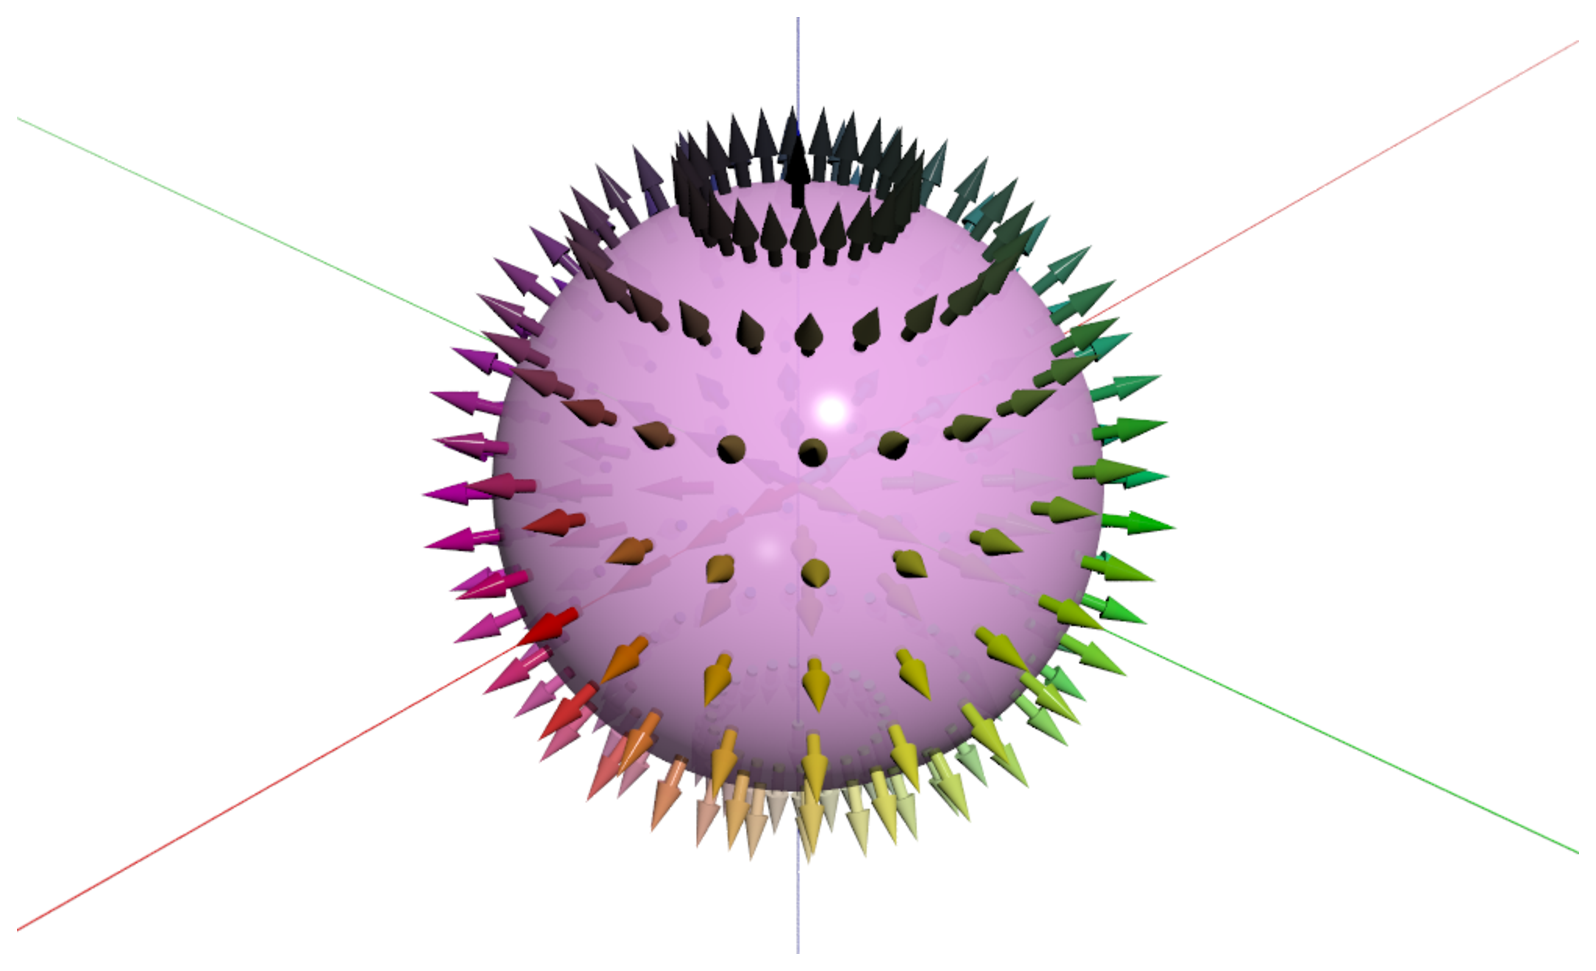
\includegraphics[width=0.55\textwidth]{Figures/blochpoint.eps}
	\caption{Illustration of a Bloch point in real space with all magnetic moments
	pointing out of the center of the Bloch sphere.
	We use the same magnetic configuration but invert the spin direction so that all moments point
	into the center.	}
	\label{fig:mnge_blochpoint}
\end{SCfigure}
In this context we perform a comparison of the Bloch point (BP) state 
and the ferromagnetic (FM) state.
The BP texture is defined by means of the four spherical parameters $\phi$, $\theta$, 
$\Phi$ and $\Theta$.
$\phi$ and $\theta$ designate the position of an \textbf{individual atom} in the unit cell
which is described by the radius $r$ and the common polar and azimuthal angle
\beq
\phi = \arctan{\left(y/x\right)}
\eeq
and
\beq
\theta = \arccos{\left( \frac{z}{\sqrt{x^2+y^2+z^2}} \right)}.
\eeq
The BP texture does not depend on $r$ and we can therefore neglect it in the following.
Usually, the atomic positions are given in the Cartesian coordinates $x,y$ and $z$.
In the definition above, we define the origin of the coordinate system, \textit{i.e.}, the tuple $(x=0, \, y=0, \, z=0)$,
to be at the center of the unit cell.
In this frame of reference, all atoms that lay in an x-y-plane that intersects with the center
are described by $\theta=\pi/2$.
The orientation of the \textbf{individual atomic magnetic moments} for a BP texture is then defined 
by the polar angle
\beq
\Phi = \phi + \phi_{1}
\eeq
and the azimuthal angle
\beq
\Theta = 2 \arctan{\left(\cot{\frac{\theta}{2}} \right)},
\eeq
where the angles designating the atomic position enter as arguments. $\phi_{1}$ is a phase factor.
An illustration of a BP is given in \cref{fig:mnge_blochpoint}. Note, that in contrast to
that illustration we conduct our investigation for a BP with $\phi_{1}=\pi$, where magnetic moments
are inverted, \textit{i.e.}, all moments point into instead of out of the center.
\\
For our calculations we
again use a $6\times 6\times 6$ supercell but this time with a $2\times 2\times 2$ k-point-mesh and LDA as
exchange-correlation functional. Here, we choose LDA because it has been used extensively in all KKR codes
in the past and 
we want to eliminate the possibility of numerical problems that could occur when SOC is artificially enhanced.
The magnetic moments are allowed to relax during the convergence process.
This leads to a small canting of the moments which is a known effect in
B20 materials \cite{chizhikov_multishell_2013}.
\begin{figure}[!htb]
  \centering
   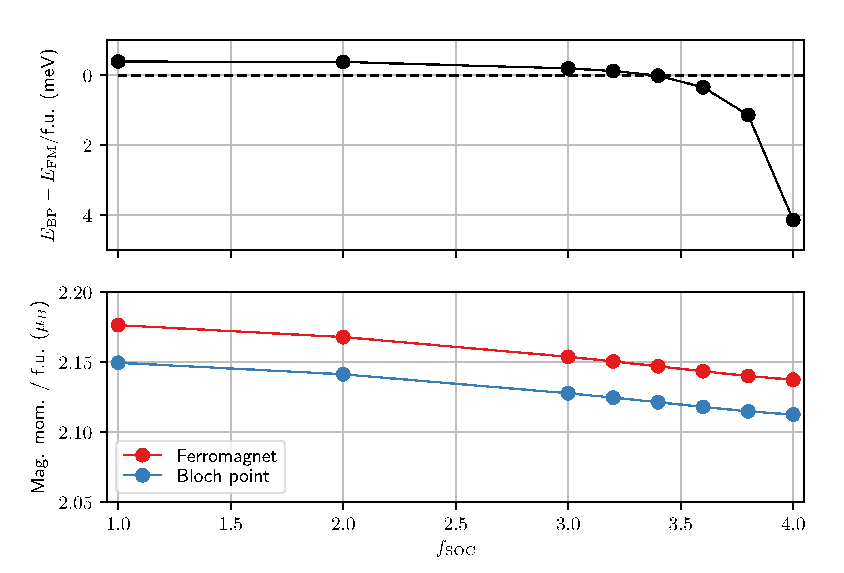
\includegraphics[width=1.00\textwidth]{Figures/MnGe_ferro_bp.eps}
	\caption{Effect of increased SOC on B20-\ce{MnGe} in a $6\times 6\times 6$ supercell.
	Top: Total energy difference between (relaxed) Bloch point and (relaxed) ferromagnet.
	Bottom: Magnetic moment of ferromagnet and Bloch point state.}
\label{fig:MnGe_kkrnano_comparison_bp}
\end{figure}
A series of calculations is conducted ranging from the physical value of the SOC 
to
an enhancement of it by a
factor of $f_{\text{SOC}}=4.0$ (see \cref{fig:MnGe_kkrnano_comparison_bp}).
As could be expected from the investigation of 1Q and 3Q state before,
the BP state is energetically not preferred over the FM state for a small
scaling of SOC.
However, when SOC is scaled further up to $f_{\text{SOC}}=3.5$,
both states are energetically more or less equivalent.
Above $f_{\text{SOC}}=3.5$ the BP state is clearly preferred over the FM state with
an energy difference of up to 4 meV/f.u.
Within the parameter range that we checked in this study,
the most beneficial scaling value for the BP is found to be $f_{\text{SOC}}=4.0$.
The effect of SOC scaling on the magnetic moment can be deemed negligible. Over the whole
range it decreases by 0.07 $\mu_{B}$ for each of the two states
(see again \cref{fig:MnGe_kkrnano_comparison_bp}).
It would be interesting to check whether a global minimum of $E_{\text{BP}}-E_{\text{FM}}$ can
be found for $f_{\text{SOC}} > 4.0$. This would hint to an optimal
scaling at which also other non-collinear magnetic textures, e.g., 1Q spin spiral or
3Q hedgehog lattice, can possibly be stabilized.
However, this is not possible as our method becomes increasingly numerically unstable for 
such strong scaling factors, i.e., the total energy does not converge anymore.
The reason for this is currently under investigation.

\FloatBarrier

\section{Justification of Extension}
As shown in the previous section, there are promising hints for the existence of non-trivial magnetic textures in
B20-\ce{MnGe} that can be found not only in experiment but also in \textit{ab initio} calculations with KKRnano.
However, the obvious approach of imposing the experimentally reported magnetic texture on the system does not
confirm the existence of a 1Q or 3Q ground state unless parameters like the lattice constant and the strength of 
spin-orbit coupling are adjusted.
It is our aim to verify the existence of non-trivial ground states without such adjustments and hence
we spent a considerable amount of time on the investigation of B20-\ce{MnGe} employing other variants
of the KKR method
to extract microscopic
parameters to construct an extended Heisenberg model that is used to detect magnetic phase transitions and
to perform Atomistic Spin Dynamics (ASD) simulations. Here we noticed that due to the low-symmetry 
position of the magnetic 
atoms a canting of the atoms can emerge that goes beyond that what could be resolved experimentally so far. 
Thus, we plan to continue along the path of finding the magnetic structure of B20-MnGe, but adjusting our scheme, 
\textit{i.e.}\  we would like to look into an improved quantitative description of the magnetization given in
\cref{eq:3q_formula} and \cref{eq:1q_spiral} by accounting for the aforementioned canting effect and
other effects that arise from higher-order terms in the extended Heisenberg Hamiltonian.
Apart from these challenges, that are related to nature of the underlying physics,
Hazel Hen has been very busy and pretty occupied throughout the current accounting period.
This prohibited us from obtaining results in a timely manner as mid-sized computing jobs of 50-100 nodes
were almost always queued for a couple of days and occasionally even for more than a week.


\bibliography{references}

%\section{Bibliographic References}
%\rule{\textwidth}{0.4pt}\\
%\textit{Provide recent/most important bibliographic references that are relevant to the project.}\\

%\bigskip
%\begin{flushright}
%{\tiny V1.3-2016JUN07}
%\end{flushright}
\end{document}
